
\chapter{Evaluación\label{chap:Evaluaci=0000F3n}}

En este capitulo se presenta la evaluación del enfoque propuesto con
el objetivo de analizar el desempeño de las técnicas de aprendizaje
de maquina para predecir propiedades no-funcionales en dispositivos
móviles. Con este fin, se crearon tres diferentes casos de estudio
sobre los que se aplica y analiza el enfoque.

El capítulo se organiza de la siguiente manera: en la sección \ref{sec:Metodolog=0000EDa-de-Evaluaci=0000F3n}
se detalla la metodología de evaluación propuesta para analizar la
eficacia de los modelos de predicción, se incluye información complementaria
sobre las métricas usadas, el formato de los resultados obtenidos,
los criterios empleados para la configuración de los parámetros de
cada técnica y las características de los dispositivos móviles usados
para las pruebas. En la sección \ref{sec:Escenarios} se presentan
los escenarios de estudio considerados, brindando una descripción
de los dataset obtenidos junto a gráficas y análisis sobre la distribución
de los datos, con el fin de comprender mejor el desempeño de las técnicas
de regresión analizadas. Los resultados obtenidos son expuestos en
la sección \ref{sec:Resultados-y-discusi=0000F3n} desglosados por
escenario para analizar el desempeño de las técnicas sobre cada dominio.
Finalmente en la sección \ref{sec:Conclusiones} se presentan las
conclusiones del capítulo. 


\section{Metodología de Evaluación\label{sec:Metodolog=0000EDa-de-Evaluaci=0000F3n}}

La calidad de los modelos será evaluada a través de seis métricas
de regresión que representan de forma distinta el error de predicción.
Así mismo, para un análisis más profundo sobre las distintas técnicas
y su desempeño se usaron cuatro escenarios o contextos dispares entre
sí para determinar, de ser posible, las técnicas que mejor se adecuan
a un escenario (por su naturaleza), o por el contrario, no aplican
adecuadamente ante un escenario particular. 

Cada modelo es definido por una técnica \emph{X} (regresión lineal,
red neuronal, etc.) que se aplica para predecir una propiedad \emph{Y},
(tiempo de respuesta y precisión) de un componente \emph{Z}. 

En todos los escenarios se considera el tiempo de respuesta como propiedad
a predecir, y sólo en aquellos donde el contexto lo permitía se incorporó
como propiedad la optimad o precisión en el resultado arrojado por
el componente. 


\subsection{Métricas de evaluación\label{subsec:M=0000E9tricas-de-evaluaci=0000F3n}}

Existe una gran cantidad de métricas por las cuales pueden evaluarse
y compararse los modelos de regresión. Todos los indicadores comparan
los valores reales con sus estimaciones, pero lo hacen de una manera
ligeramente diferente. 

\emph{\ac{MAE}} representa el promedio del error absoluto (diferencia
entre los valores predichos y los observados), e indica cuán grande
es el error que puede esperarse de la predicción. Al tratarse de una
métrica basada en el error medio puede subestimar el impacto de errores
grandes pero infrecuentes. Si el análisis se centra demasiado en la
media arrojará conclusiones precipitadas, por lo tanto para ajustar
errores grandes y raros, se calcula el error cuadrático medio (\ac{RMSE}).
Mediante la cuadratura de los errores en lugar de la media y luego
tomar la raíz cuadrada de la media, se llega a una medida del tamaño
del error que da más peso a los errores grandes e infrecuentes que
la media. 

La comparación entre las métricas \emph{\ac{RMSE} }y \emph{\ac{MAE}
}puede ser útil para determinar si un dataset contiene errores significativos
y poco frecuentes, cuanto mayor sea la diferencia entre ambos indicadores,
más inconsistente es el tamaño del error.

El coeficiente de correlación (\ac{CC}) es analizado en conjunto
con el indicador \emph{\ac{RMSE}} ya que existe una estrecha relación
entre ambos. Por ejemplo, si \emph{\ac{CC}} es 1, \emph{\ac{RMSE}}
debe ser 0, ya que todos los puntos se encuentran en la línea de la
función de regresión; cuanto más cercano sea el valor de \emph{\ac{CC}}
a 1 o -1, más próximos son los valores observados a la línea de predicción,
y por tanto menor será el error absoluto reflejado en \emph{\ac{RMSE}}. 

Por otro lado, complementariamente se utilizan indicadores relativos
en lugar de absolutos como los descriptos anteriormente, ya que ponderan
el error de predicción respecto a la variación estándar de las observaciones.
De esta manera se obtienen indicadores \emph{\ac{RAE}} y \emph{\ac{RRSE}}
de valores entre 0 y 1 para obtener una visión de las observaciones
respecto a la media. 


\subsection{Parámetros de configuración de las técnicas\label{subsec:Par=0000E1metros-de-configuraci=0000F3nde}}

La optimización y posterior obtención de un modelo de calidad tiene
lugar a partir del establecimiento de diversos parámetros de configuración. 

Estos parámetros pueden requerir distintos valores adaptándose a condiciones
particulares de los datos que optimicen el resultado de la predicción.
Para brindar más detalle de estos parámetros, el Cuadro \ref{tab:Par=0000E1metros-de-configuraci=0000F3n}
presenta la lista completa de parámetros propios de cada técnica,
el valor por defecto adoptado para cada una y el rango de valores
establecido con el cual se determinará el mejor valor resultante. 

\begin{table}[H]
\begin{centering}
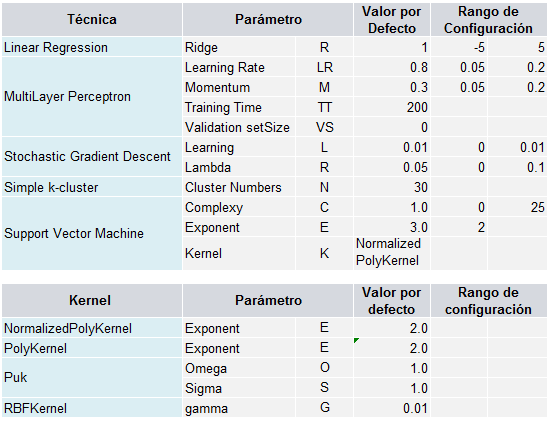
\includegraphics[scale=0.5]{C:/Users/usuario/Tesisworkspace/Tesis_Standalone/tesis/images/configuration-parameters}
\par\end{centering}

\caption{Parámetros de configuración de las técnicas de regresión \label{tab:Par=0000E1metros-de-configuraci=0000F3n}}
\end{table}


El proceso de optimización de las técnicas utiliza el rango de configuración
establecido para iterar en pasos tomando valores intermedios y evaluando
la calidad de la técnica con tales configuraciones, finalmente se
contrastan entre sí y se determina la mejor configuración para un
dataset y atributo a predecir particular. 

Los rangos para cada técnica se establecieron tras un análisis exhaustivo
de la influencia de estos valores sobre los datos. Los rangos de prueba
se definieron de manera aleatoria en conjunto de fundamentos teóricos
asociados a cada técnica, al mismo tiempo que el análisis de un rango
ya propuesto servía como base para definir uno nuevo. Los análisis
se llevaron a cabo sobre 20 archivos dataset dispuestos para esta
tesis. 

Por otro lado, los valores elegidos por defecto fueron tomados de
los valores propuestos por la herramienta Weka, a excepción del parámetro
\emph{Training Time} de la técnica \emph{MultiLayer Perceptron} que
fue reducido de 500 a 200 para mejorar la performance de tiempo del
algoritmo. 

Para el caso de la técnica \emph{Support Vector Machine} la configuración
es más compleja ya que involucra parámetros propios simples y un kernel
con parámetros específicos. Para la técnica \emph{\ac{SMO}}, el parámetro
\emph{gamma} y \emph{complexy} fueron analizados en conjunto con el
apoyo de fundamentos teoría y empíricas. La figura \ref{fig:RBF-parameters-SVM}
refleja el impacto que tienen los parámetros sobre la clasificación
de los datos. 

\begin{figure}[H]
\begin{centering}
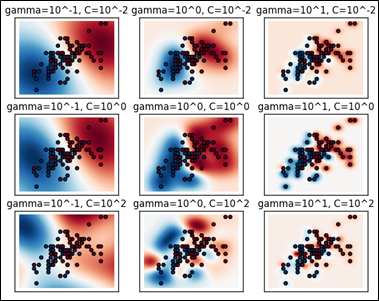
\includegraphics[scale=0.55]{C:/Users/usuario/Tesisworkspace/Tesis_Standalone/tesis/images/RBF-parameters-SVM}
\par\end{centering}

\caption{Efecto de los parámetros de la técnica SVM. \label{fig:RBF-parameters-SVM}}
\end{figure}


Las mejores opciones para configurar los parámetros se obtienen observando
la diagonal en donde los valores se incrementan a la par, la primer
imagen de la cuadrícula aplica una clasificación muy simple sobre
los datos, dejando en evidencia un alto grado de error en las predicciones.
La última imagen, en cambio, muestra un claro ejemplo de \emph{overfit},
por lo que no resulta ser una buena opción a la hora de buscar generalización.
La imagen central resulta entonces, ser la más apropiada para definir
los valores por defecto para estos parámetros. Por otro lado, la optimización
para el parámetro \emph{complexy} se determinó bajo el rango 0 - 25
debido a pruebas empíricas realizadas sobre el conjunto base de dataset. 

Respecto a la optimización del kernel, los cuatro algoritmos considerados
fueron analizados mediante la técnica prueba y error y de esa forma,
se determinaron los valores por defecto para los parámetros propios
de cada uno. Del análisis se desprenden algunas conclusiones consecuentes: 
\begin{description}
\item [{Normalized~Polynomial}] El valor por defecto para el parámetro
\emph{exponent} es 2.0 y hasta valores de 5.0 los resultados esperados
son buenos. 
\item [{Poly~Kernel}] El valor por defecto para el parámetro \emph{exponent}
es 1.0. Si el valor se incrementa se obtienen mejores resultados,
sin embargo para valores mayores a 5.0 el error de predicción comienza
a aumentar gradualmente. 
\item [{Puk}] El valor por defecto para el parámetro \emph{omega} es 1.0,
la modificación de este valor es indiferente a los resultados por
lo que no aplica a la optimización. Respecto a \emph{sigma} se adopta
el valor 0.01 ya que el incremento en este valor no produce buenos
resultados. 
\item [{RBF}] Partiendo de un valor \emph{gamma} de 0.01 se obtienen buenos
resultados, e incluso incrementando este valor a razón de 0.01 los
resultados tienden a mejorar. 
\end{description}

\subsection{Características de los dispositivos móviles usados\label{subsec:Caracter=0000EDsticas-de-los}}

En la mayoría de las pruebas se han utilizado dos dispositivos móviles,
el modelo K3 Note de la marca Lenovo y el modelo Galaxy S3 de la marca
Samsung.

También se utilizaron tres modelos más sólo para el escenario del
problema del viajante. Todas las especificaciones son expuestas en
el cuadro \ref{tab:Especificaciones-de-los}. 

\begin{table}[H]
\resizebox{.80\textwidth}{!}{%
\begin{tabular*}{20cm}{@{\extracolsep{\fill}}|c|c|c|c|c|}
\hline 
\selectlanguage{english}%
\selectlanguage{english}%
 & CPU Procesador/Núcleos & GPU tarjeta gráfica & Memoria RAM & Sistema Operativo\tabularnewline
\hline 
Lenovo K3 & 1.7Ghz Octa-Core ARM Cortex-A53 & ARM Mali-T760 MP2 & 2GB LPDDR3 & Android 5.0\tabularnewline
\hline 
Samsung Galaxy S3 & Quad-Core 1.4 Ghz Cortex-A9 & Mali-400MP & 1GB & Android 4.3\tabularnewline
\hline 
Samsung Galaxy S4 & Qualcomm APQ8064T Snapdragon 600 1.9Ghz /4 & PowerVR SGX 544MP / Adreno 320 & 2GB & Android 4.2.2\tabularnewline
\hline 
Samsung Galaxy S5 & Qualcomm MSM8974AC Snapdragon 801 2.5Ghz /4 & Adreno 330 & 2GB & Android 4.4.2\tabularnewline
\hline 
Samsung Galaxy S6 & 2.1Ghz Samsung Exynos /8 & Mali-T760 & 3GB LPDDR4 & Android 5.0\tabularnewline
\hline 
\end{tabular*}}

\caption{Especificaciones de los dispositivos móviles utilizados. \label{tab:Especificaciones-de-los}}
\end{table}



\section{Escenarios\label{sec:Escenarios}}

Definidas las métricas, la metodología de evaluación y los parámetros
de configuración, en la presente sección se detallarán los escenarios
sobre los que se aplica el enfoque. Por cada escenario se describen
los componentes involucrados, el proceso de medición de los mismos
y un análisis de los datos obtenidos, formando un dataset particular
para evaluar las tecnicas de regresión. 


\subsection{Escenario 1: Multiplicación de matrices\label{subsec:Escenario-4:-Multiplicaci=0000F3n}}

El producto de matrices corresponde a problemas de clase P ya que
a diferencia de los problemas NP, su complejidad es polinómica. El
producto entre matrices no es conmutativo, depende del orden de las
matrices intervinientes y su multiplicación sólo es posible si el
número de filas de la primera matriz es igual al número de columnas
de la segunda. 

Los dataset para este dominio han sido formados tras la ejecución
de diferentes algoritmos de multiplicación de matrices, con tamaños
variados de matrices. Existen dos clases de datasets, aquellos que
involucran el component RenderScript y aquellos que lo excluyen. Para
el primer caso se generaron 894 instancias lo cual comprende un total
de 149 entradas por componente. Para el segundo caso, el dataset se
compone de 745 instancias. 

Los componentes o algoritmos considerados para este dominio se describen
a continuación: 
\begin{description}
\item [{Matrix~Multiplication}] implementación simple desarrollada puramente
en lenguaje Java. 
\item [{Matrix~Multiplication~Multi~Thread}] corresponde a la misma
versión del componente anterior paralelizada en ocho threads de ejecución. 
\item [{Matrix~Multiplication~Render~Script}] es una versión implementada
con RenderScript , de modo que si el dispositivo tiene un \ac{GPU}
compatible con RenderScript, éste lo ejecutará. Por tal razón el tiempo
de operación es mucho más rápida. 
\item [{Native~Matrix~Multiplication}] es una versión que usa \ac{JNI}
para que la multiplicación se realice sobre código nativo desarrollado
en lenguaje C++, el cual se compila específicamente según cada arquitectura
de \ac{CPU} (Armeabi, x86, etc). 
\item [{Matrix~Multiplication~with~Eigen}] versión que usa \ac{JNI}
para ejecutar la multiplicación de matrices provista por la librería
nativa Eigen. 
\item [{Matrix~Multiplication~with~OpenCV}] versión que usa \ac{JNI}
para ejecutar la multiplicación a través de la librería OpenCV . 
\end{description}
Las entradas del problema utilizadas para la evaluación fueron generadas
aleatoriamente a partir de las dimensiones (tamaño) de las matrices
involucradas a partir del número de filas y columnas de la primer
matriz denominada matriz A y el número de columnas de la segunda matriz
denominada matriz B, esta distinción es importante teniendo en cuenta
la propiedad de no conmutabilidad del producto de matrices. Adicionalmente,
ambas matrices pueden ser configuradas externamente. De cada instancia
del problema, las entradas que se tomaron en cuenta fueron: el número
de columnas de la primer matriz (\emph{AColumn}), el número de filas
y el de columnas de la segunda matriz (\emph{ARow} y \emph{BColumn}).

Por último, el dataset incluye atributos de la ejecución del componente;
la complejidad temporal de la operación definida como O(AColumn x
ARow x BColumn) y el tiempo de respuesta de la operación registrada
en segundos. No fueron incluidos atributos relativos al dispositivo
de ejecución, sin embargo podrían considerarse propiedades como número
de cores de \ac{CPU}, cores de \ac{GPU}, frecuencia, etc. ya que
se piensa son buenos predictores de tiempo para algunos algoritmos. 

Las pruebas fueron ejecutadas sobre 2 modelos de dispositivos móviles,
Lenovo K3 y Samsung Galaxy S3. Lo interesante de este dataset, es
que los algoritmos fueron implementados con diferentes librerías y
diseñados para ser ejecutados por diferente elementos de hardware
(\ac{CPU}, \ac{GPU}, etc). 

A continuación en la figura \ref{fig:matrix-dataset-behaviour} se
muestra el comportamiento del atributo \emph{Tiempo de respuesta}
de los dataset formados para este dominio, en referencia a la imagen,
A) Sin componente RenderScript en Lenovo K3, B) Sin componente RenderScript
en Samsung Galaxy S3, C) Todos los componentes en Lenovo K3 y D) Todos
los componentes en Samsung Galaxy S3.

\begin{figure}[H]
\begin{centering}
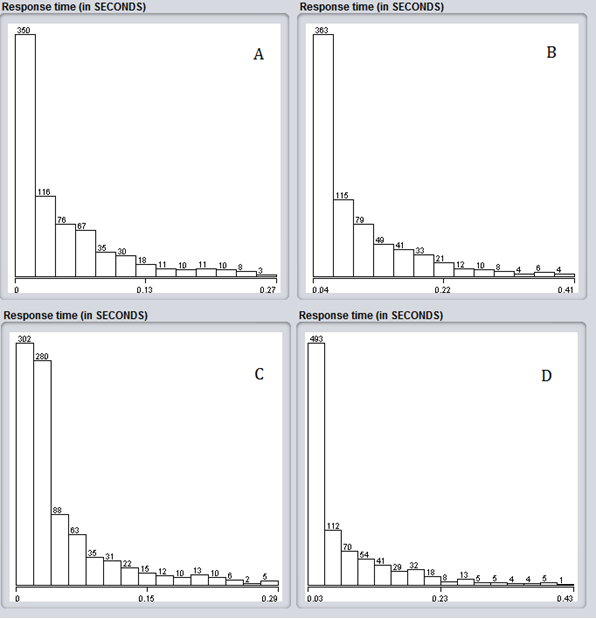
\includegraphics[scale=0.55]{C:/Users/usuario/Tesisworkspace/Tesis_Standalone/tesis/images/matrix-dataset-behaviour}
\par\end{centering}

\caption{Comportamiento del atributo ‘Tiempo de respuesta’ para el problema
de la multiplicación de matrices.\label{fig:matrix-dataset-behaviour}}
\end{figure}


En todos los casos puede observarse una distribución exponencial de
los datos incluyendo valores extremos o infrecuentes. Respecto a los
valores de tiempo registrados, puede notarse a simple vista que las
pruebas ejecutadas en el dispositivo Lenovo K3 consumen menor tiempo
en contraste con el dispositivo Samsung Galaxy S3. 

Lo interesante de este escenario es que permite la creación de modelos
simples, por ejemplo, a partir de la técnica Linear Regression que
arroje los mismos o mejores resultados que otras técnicas más complejas
ya que entre los términos de la función de predicción se expresa la
complejidad del algoritmo de matrices. Incluso, se podrían usar técnicas
específicas para cada componentes evaluando y analizando el impacto
sobre la predicción. Por ejemplo, para el componente \emph{Multiplicación
MultiThread} en la técnica Linear Regression puede considerarse el
número de threads; para el componente con RenderScript puede considerarse
alguna característica propia del \ac{GPU} donde se ejecuta si implica
alguna mejora en los resultados predictivos. 


\subsection{Escenario 2: Algoritmos para el problema del viajante\label{subsec:Escenario-1:-Algoritmos}}

En el campo de la teoría de complejidad computacional, el problema
del viajante o \ac{TSP} por sus siglas en inglés, es tratado como
un problema NP-Completo y es modelado como un grafo de manera que
las ciudades son sus vértices, los caminos son las aristas y las distancias
entre caminos son los pesos de las aristas. Es un problema de minimización
tras la búsqueda de un recorrido completo que comienza y finaliza
en un vértice específico y visita el resto de los vértices exactamente
una vez con coste mínimo. Existen muchas variantes del problema, una
de ellas se trata del \ac{TSP} simétrico en el cual la distancia
entre un par de ciudades es la misma en cada dirección formando un
grafo ponderado no dirigido. Esta variante fue la versión considerada
por la herramienta. 

Los dataset para este dominio han sido formados tras la ejecución
de algoritmos de resolución del problema del viajante. Se generaron
archivos de entrenamiento compuestos por 192 instancias, considerando
32 entradas por componente.

Los componentes o algoritmos considerados para este dominio se describen
a continuación: 
\begin{description}
\item [{Best~Fit}] algoritmo heurístico que selecciona las ciudades de
acuerdo al costo de sus trayectos y son incorporadas al conjunto Solución
en base al cálculo de la distancia marginal de las intersecciones.. 
\item [{Nearest~neighbour}] partiendo de alguna ciudad arbitraria se analizan
todos los vértices adyacentes y aún no visitados, y se añade a la
solución aquel vértice cuya arista de costo sea la mínima. 
\item [{Lineal~Programming}] realiza una búsqueda exhaustiva simulando
el algoritmo backtracking, considerando restricciones y funciones
objetivo como fórmulas matemáticas. 
\item [{Prim}] crea un árbol de recubrimiento sobre el grafo y crea un
ciclo euleriano mínimo
\item [{Kruskal}] algoritmo similar a Prim en funcionamiento pero no en
ejecución, variando su complejidad.
\item [{Local~Transformations}] A través de un grafo hammiltoniano, se
analizan las aristas cruzadas obteniendo un nuevo ciclo.
\end{description}
Con el fin de garantizar instancias variadas del problema (diferentes
cantidades de ciudades, distintas representaciones y pesos) y para
la medición de los componentes, se utiliza la librería TSPLib que
contiene archivos con múltiples instancias del problema.. La librería
cuenta con 111 archivos de formato TSP, y 32 archivos de formato OPT.TOUR
que contienen el recorrido óptimo del archivo que referencian. Los
ejemplos oscilan desde 14 y hasta 18512 ciudades con un sólo ejemplo
extremo de 85900, y utilizan cuatro funciones de cálculo de la distancia
entre ciudades: distancia euclidiana, distancia geométrica, distancia
pseudo euclidiana y función techo. Para la obtención de las mediciones
correspondientes, se realizó una pre selección de 32 archivos que
comprenden ejemplos de entre 22 y 200 ciudades. Cabe destacar que
fue necesaria la implementación de un parser para el uso de los archivos. 

Por último, el dataset incluye atributos de la ejecución del componente;
exactitud y precisión en el resultado, tiempo de respuesta y valor
solución. En cuanto a la precisión y exactitud de las respuestas se
consideraron tres indicadores que toman en cuenta las repeticiones
en la respuesta y la totalidad o falta de los vértices incluidos.
El indicador TP (\emph{true positive}), para los vértices incluidos
en la solución, FP(\emph{false positive}), para las repeticiones de
vértices y FN (\emph{False Negative}) para los vértices no incorporados
en la solución. Por lo tanto, se consideró: 

\[
Precisi\acute{o}n=\frac{TP}{FP+TP}
\]


\[
Exactitud=\frac{TP}{FP+TP+FN}
\]


A modo de ejemplo, se presenta en la figura \ref{fig:TPS-graph-problem}
un grafo con comienzo en la ciudad A. Suponiendo que un algoritmo
de resolución arroja el siguiente camino solución: \{A, B, D, A\},
se obtiene una precisión del 100\% al tener un valor de \ac{TP} =
3 y un valor de \ac{FP} = 0 ya que no hay vértices repetidos en la
solución, sin embargo, la solución no es correcta ya que no incluye
la totalidad de vértices del conjunto (excluye al vértice C). En cambio,
al calcular la exactitud se obtiene un valor del 66\% al tener un
valor de \ac{TP} = 4, \ac{FP} = 1 y \ac{FN} = 1 brindando un concepto
más realista. 

El uso del indicador de precisión o el de exactitud dependerá del
contexto en el que se aplique. 

\begin{figure}[H]
\begin{centering}
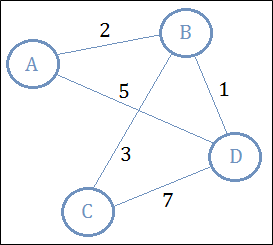
\includegraphics[scale=0.55]{C:/Users/usuario/Tesisworkspace/Tesis_Standalone/tesis/images/TPS-graph-problem}
\par\end{centering}

\caption{Ejemplo de grafo para el problema del viajante.\label{fig:TPS-graph-problem}}
\end{figure}


Las pruebas fueron llevadas a cabo sobre los dispositivos móviles
Samsung Galaxy S4, S5 y S6.

El objetivo de este escenario es la creación de modelos capaces de
predecir el tiempo de respuesta de cada algoritmo frente a distintas
características de las entradas, y modelos para predecir la calidad
en los caminos retornados. En la figura \ref{fig:TPS-dataset-behaviour}
expuesta a continuación se muestra el comportamiento del conjunto
de mediciones.

\begin{figure}[H]
\begin{centering}
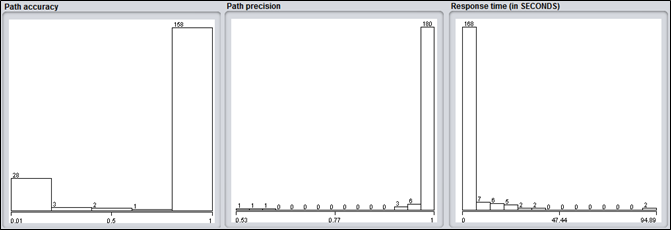
\includegraphics[scale=0.55]{C:/Users/usuario/Tesisworkspace/Tesis_Standalone/tesis/images/TPS-dataset-behaviour}
\par\end{centering}

\caption{Comportamiento del dataset para el escenario del problema del viajante.\label{fig:TPS-dataset-behaviour}}
\end{figure}


A primera vista la figura \ref{fig:TPS-dataset-behaviour} permite
observar una gran concentración de datos sobre los extremos para los
valores de precisión y tiempo de respuesta. En el primer caso, aproximadamente
un 94\% de los datos toman el valor 1, y en el segundo caso, un 88\%
de los datos toman valores entre 0 y 6.77 segundos. Este comportamiento
uniforme y poco distribuido de los datos obstaculiza el desarrollo
de un buen modelo predictivo. 

Respecto al atributo \emph{accuracy}, si bien presenta más dispersión
entre los datos, aproximadamente un 82\% circunda alrededor del valor
1 y un 15\% sobre valores cercanos a 0.008. 


\subsection{Escenario 3: Servicios para detección de rostros\label{subsec:Escenario-2:-Servicios}}

El segundo escenario comprende un conjunto de servicios Web para la
detección de rostros en imágenes. Hoy en día muchas soluciones para
detección de rostro se proporcionan como servicios Web, que aunque
no son tan rápidos y usables sin conexión a Internet como las bibliotecas
de software, resultan generalmente más precisos y proporcionan características
muy peculiares del rostro. Sin embargo, el rendimiento y la precisión
de los servicios varían según las propiedades de la imagen (tamaño,
foco, oclusiones) y contexto de ejecución (capacidad de la \ac{CPU},
conexión de red).

Los dataset para este dominio han sido formados tras la ejecución
de diferentes servicios para detección de rostros en imágenes. Los
dataset son particulares a cada servicio, y se conforman por diferente
cantidad de entradas e instancias.

Los componentes involucrados incluyen un servicio o proceso Android
(Google Play Services (GMS) face detector) y tres servicios Web (FaceRect
API, Sky Biometry API y Microsoft Face API). 

A continuación se detallan las principales características de los
servicios (componentes contemplados):


\paragraph{GMS}

La compañía Google ha implementado una colección extensa y variada
de aplicaciones para Android. Entre ellas, ofrece el paquete ‘com.google.android.gms.vision’
el cual proporciona una funcionalidad común para trabajar con detectores
de objetos visuales. En la figura \ref{fig:GooglePlay-services}se
muestra la forma en que el objeto \emph{GoogleAPIClient} proporciona
una interfaz para conectar y hacer llamadas a cualquiera de los servicios
de Google Play disponibles tales como Google Play Games, Google Drive,
Google Maps, etc 

\begin{figure}[H]
\begin{centering}
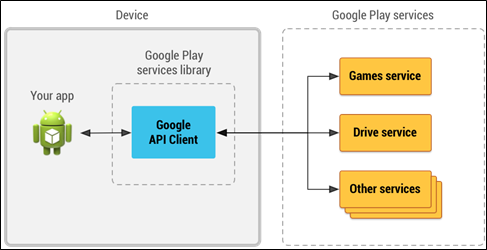
\includegraphics[scale=0.55]{C:/Users/usuario/Tesisworkspace/Tesis_Standalone/tesis/images/GooglePlay-services}
\par\end{centering}

\caption{Esquema conceptual para el uso de servicios de Google Play Services.\label{fig:GooglePlay-services}}


\selectlanguage{english}%
\selectlanguage{english}%
\end{figure}


El algoritmo permite setear tres parámetros diferentes (\emph{allLandmarks}
, \emph{allClassifications} , \emph{accurateMode}) dando lugar a 8
configuraciones posibles por imagen. Para el servicio GMS se utilizaron
290 imágenes originando un dataset de 2320 instancias. 


\paragraph{FaceRect API y Sky Biometry API}

Los servicios web \emph{SkyBiometry} y \emph{FaceRect} son consumidos
directamente desde la aplicación online \emph{Mashape}, la cual ofrece
una gran variedad de aplicaciones, incluida una colección de Aplicaciones
sobre detección y reconocimiento de rostros. SkyBiometry y FaceRect
son aplicaciones que utilizan interfaz REST, es decir, los métodos
son llamados a través de Internet usando los métodos \ac{HTTP} estándar
como GET y POST a las direcciones correspondientes. Dependiendo de
los parámetros especificados en el request, el servidor puede generar
la respuesta tanto en formato \ac{JSON} como \ac{XML}. Adicionalmente,
se utilizó el servicio GMS Visión de Google a partir de la librería
correspondiente. Los tres servicios son descritos en detalle en el
apéndice B.

El algoritmo de la aplicación FaceRect permite setear sólo una opción
(\emph{features}) por imagen, de modo que se construyó un dataset
con sólo dos propiedades, incluyendo el tiempo de respuesta y un total
de 54 instancias. 

Por otro lado, el algoritmo de Sky Biometry permite setear siete parámetros
diferentes dando lugar a 128 configuraciones posibles por imagen (\emph{aggressive},
\emph{gender}, \emph{glasses}, \emph{smiling}, \emph{mood}, \emph{age},\emph{
eyes}). Para el servicio Sky Biometry se utilizaron 30 imágenes originando
un dataset de 3840 instancias y se incluyen 8 propiedades, además
de los parámetros configurables del tipo binario se añade el tiempo
de respuesta. 


\paragraph{Microsoft Face API}

Face API es un servicio web en la nube que provee los algoritmos de
detección y reconocimiento de rostros más avanzados. El servicio es
consumido a través del sitio de Microsoft y las respuestas son retornadas
en formato \ac{JSON}. El algoritmo permite setear seis propiedades
(\emph{landmarks}, \emph{age}, \emph{gender}, \emph{facialHair}, \emph{smile}
y \emph{headPos}). El dataset está formado por 1826 instancias y siete
propiedades, además de los parámetros configurables como atributos
binarios se incluye el tiempo de respuesta. 

Estos cuatro componentes fueron evaluados a partir de subconjunto
de 290 imágenes pertenecientes al dataset llamado FDDB \citep{fddbTechReport}
con características muy variadas. Cada servicio es llamado especificando
una imagen y un conjunto de parámetros booleanos (a través del valor
0 y 1) que determinan las funciones requeridas del algoritmo determinado.
En los cuatro servicios, el tiempo de respuesta es una variable continua
y registrada en mili segundos. 

Cabe destacar que las pruebas fueron realizadas en un único dispositivo
móvil (Lenovo K3 Note), por tal motivo no se consideran características
propias del móvil ya que significan valores constantes en la predicción.
Por lo tanto el objetivo de este escenario es crear modelos para predecir
el tiempo de respuesta a partir de características variables de la
imagen de entrada y de los parámetros de configuración del componente
en cuestión.

En la figura \ref{fig:face-services-dataset-behaviour} que se muestra
a continuación se expone el comportamiento de los datos del atributo
\emph{Tiempo de respuesta} para cada uno de los servicios, en referencia
con la imagen A) FaceRect API, B) Microsoft Face API, C) Google Play
Service y D) Sky Biometry API. 

\begin{figure}[H]
\begin{centering}
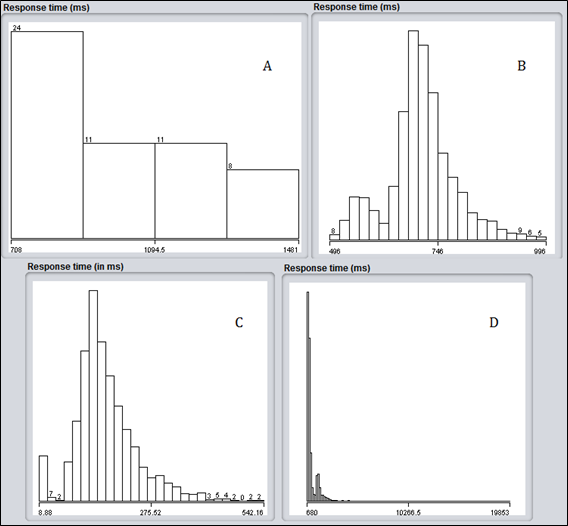
\includegraphics[scale=0.55]{C:/Users/usuario/Tesisworkspace/Tesis_Standalone/tesis/images/face-services-dataset-behaviour}
\par\end{centering}

\caption{Comportamiento del atributo ‘Tiempo de respuesta’ de los servicios
de detección de rostros.\label{fig:face-services-dataset-behaviour}}
\end{figure}


El servicio Sky Biometry presenta entre sus datos un 5\% de valores
infrecuentes y en esos casos valores extremos, siendo el único servicio
en presentar estas características. 

El servicio de Microsoft Face arrojó valores de tiempo de respuesta
uniformemente distribuidos en el intervalo tomando la forma de campana
de Gauss, los datos se distribuyen simétricamente sobre el intervalo,
es decir, no hay presencia de sesgos hacia la izquierda o hacia la
derecha. Google Play también tiene una distribución de Gauss con sesgo
hacia la izquierda. Puede observarse que presenta un intervalo muy
amplio, de modo que las propiedades configurables del algoritmo incrementan
considerablemente el tiempo de operación. Sin embargo, al contrastarlo
con el servicio de FaceRect, el mínimo de tiempo requerido por este
servicio es mucho mayor que el tiempo máximo arrojado por el de Google
Play, aún así cualquier análisis sobre el servicio FaceRect puede
ser precipitado, ya que se evaluó con un bajo número de instancias. 


\section{Resultados y discusión\label{sec:Resultados-y-discusi=0000F3n}}

En esta sección final de la evaluación se agrupan los resultados para
contrastar los escenarios entre sí con el fin de determinar relaciones
entre las técnicas, el contexto o dominio en el que se aplican y el
desempeño sobre los atributos que predicen, esto es, si la técnica
se ajusta más adecuadamente a un tipo de atributo o a otro, a modo
de inferir las conclusiones pertinentes. Además, se analizan detalles
sobre la performance del proceso de optimización de las técnicas respecto
al tiempo de cómputo que insumen y su relación con el tamaño del dataset
que procesa. 


\subsection{Resultados para el problema de la multiplicación de matrices.}

\begin{table}[H]
\begin{centering}
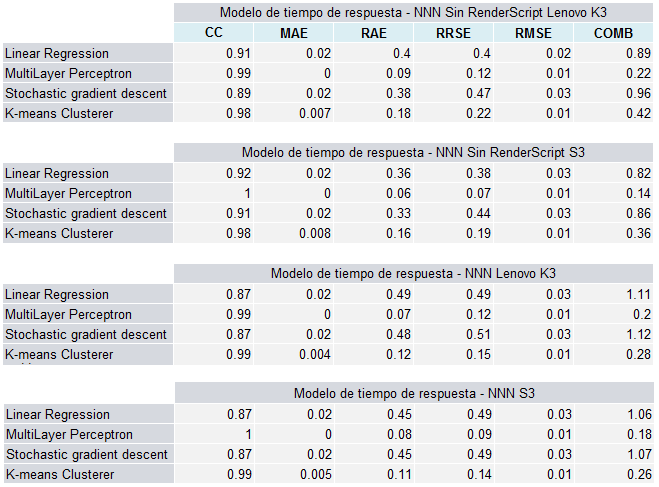
\includegraphics[bb=0bp 0bp 596bp 619bp,scale=0.55]{C:/Users/usuario/Tesisworkspace/Tesis_Standalone/tesis/images/reponse-matrix}
\par\end{centering}

\caption{Resultados del escenario ‘Multiplicación de matrices’.\label{tab:Resultados-del-response-matrix}}
\end{table}


El primer caso analizado es el problema de la multiplicación de matrices.
En el cuadro \ref{tab:Resultados-del-response-matrix} se pueden apreciar
las métricas obtenidas a partir de los modelos calculados. A simple
vista, se puede apreciar que todos los modelos obtenidos presentan
una gran correlación, significando que el atributo buscado (response
time) tiene una gran dependencia de los atributos contemplados. Esto
concluye que el tamaño de las matrices multiplicadas influye en el
tiempo de respuesta para obtener el producto de dichas matrices y
que cualquiera de los modelos estudiados funciona de forma eficiente
para este problema.

De este modo, en la figura \ref{fig:lineas-matrix-response}se presentan
las lineas de predicción para el modelo menos eficiente en cuanto
a la correlación de los datos, el \ac{SGD}

\begin{figure}
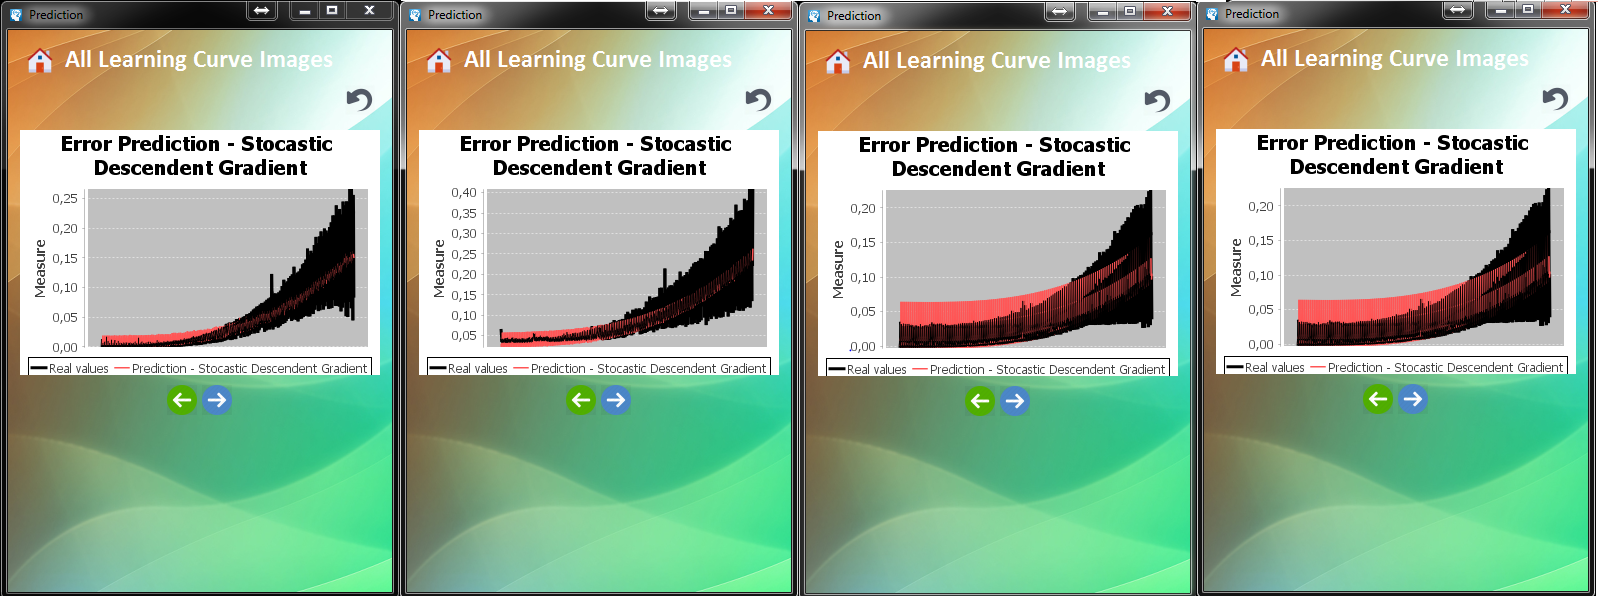
\includegraphics[scale=0.3]{C:/Users/usuario/Tesisworkspace/Tesis_Standalone/tesis/images/response_matrix_lc}

\caption{Lineas de predicción del SGD para el atributo response time\label{fig:lineas-matrix-response}}


\selectlanguage{english}%
\selectlanguage{english}%
\end{figure}



\subsection{Resultados para el problema del viajante.\label{subsec:Resultados-para-el}}

\begin{table}[H]
\begin{centering}
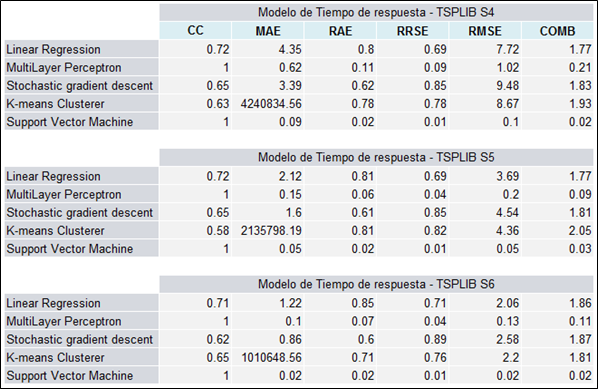
\includegraphics[bb=0bp 0bp 596bp 619bp,scale=0.55]{C:/Users/usuario/Tesisworkspace/Tesis_Standalone/tesis/images/response-TSP}
\par\end{centering}

\caption{Resultados del atributo Tiempo de respuesta para el escenario ‘problema
del viajante’.\label{tab:Resultados-del-atributo}}
\end{table}


A partir de la figura \ref{tab:Resultados-del-atributo} se desprenden
las conclusiones respecto al primer escenario. En primer punto tanto
el modelo de \emph{MultiLayer Perceptron} como el de \ac{SVM} son,
claramente, los mejores en cuanto a adaptación al modelo. Ambos presentan
una correlación de los datos de 1 (\ac{CC}), lo que representa la
exactitud de los datos predichos en relación a los reales. Como se
ha se explicado en la sección\ref{subsec:Ajuste-del-modelo:}, esto
puede parecer lo más óptimo, sin embargo observando las métricas y
las curvas de errores, ambos modelos presentan el problema de overfitting. 

Teniendo esto en cuenta, se descartan ambos modelos como los mejores
para este tipo de problemas. A su vez, se descarta el \emph{K-mean
Clusterer }ya que presenta los niveles de correlación mas bajos y
los errores más altos.

En todos los escenarios presentados, se ha optado por el caso intermedio
de adaptación, considerando que el mejor modelo obtenido será aquel
que evite casos de overfitting o underfitting, focalizando el análisis
en los valores de \ac{CC} intermedios, con un error \ac{MAE} aceptable
considerando los valores propios y errores promedios bajos. Por lo
tanto, en este caso, el modelo más eficiente es el \emph{Linear Regression.
}A continuación, se presenta el comportamiento de este último con
respecto a los valores de referencia.

\begin{figure}[H]
\begin{centering}
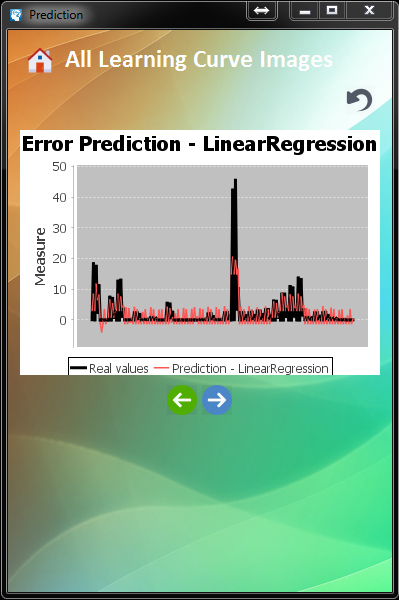
\includegraphics[scale=0.55]{C:/Users/usuario/Tesisworkspace/Tesis_Standalone/tesis/images/linear-regression-behaviour.PNG}
\par\end{centering}

\caption{Lineas de predicción en la herramienta Nekonata}
\end{figure}


Aplicando el mismo método de análisis anterior, se analizó el dataset
TSPlib.csv considerando el atributo precisión del algoritmo.

\begin{table}[H]
\begin{centering}
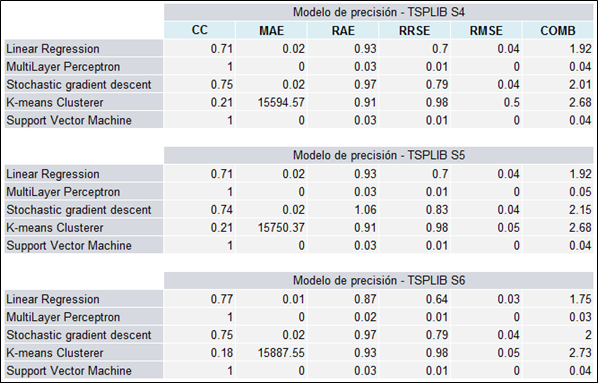
\includegraphics[bb=0bp 0bp 596bp 619bp,scale=0.55]{C:/Users/usuario/Tesisworkspace/Tesis_Standalone/tesis/images/precision-TPS}
\par\end{centering}

\caption{Resultados del atributo precisión para el escenario ‘problema del
viajante’.}
\end{table}


A través de la figura se aprecia que los modelos que presentan una
mejor adaptación para este problema continuan siendo el \ac{MLP}
y el \ac{SMO}. Aun así, considerando el análisis realizado previamente,
para el atributo precision el mejor algoritmo es el \ac{SGD}. 

Teniendo en cuenta los conceptos expuestos en la sección \ref{sub:Ajuste-del-modelo:},
el mejor algoritmo teórico que mejor se adapta al problema del viajante
es el \emph{modelo LinearRegression }es sus dos implementaciones (Ridge
y \ac{SGD}). 

\begin{figure}[H]
\begin{centering}
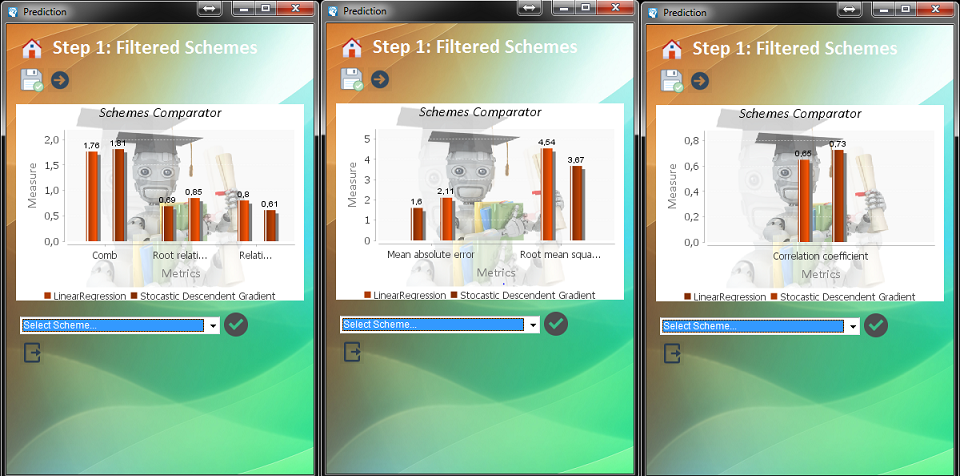
\includegraphics[scale=0.55]{C:/Users/usuario/Tesisworkspace/Tesis_Standalone/tesis/images/errors-comparison-response-S5}
\par\end{centering}

\caption{Figura comparativa de las dos implementaciones de regresión lineal
para el problema del vaiajante}
\end{figure}



\subsection{Resultados para los servicios de detección de rostros.}

Durante el proceso de formación de los dataset, se consideró en primer
medida, la incorporación de variables sobre la imagen, como el tamaño,
la intensidad de color, entre otras. Sin embargo, fueron descartadas
en la versión final ya que no demostraron influir sobre la precisión
y el tiempo de respuesta al alcanzar un grado de correlación por debajo
de 0.05 entre las variables de la imagen y las variables a predecir.
Sólo los parámetros de configuración con los que se invocan a la función
de detección de cada componente afectaron directamente al tiempo de
respuesta requerido por el servicio. Los resultados de los modelos
obtenidos para la predicción del atributo \emph{Tiempo de respuesta}
se exponen en el cuadro \ref{tab:Resultados-response-face}

\begin{table}[H]
\begin{centering}
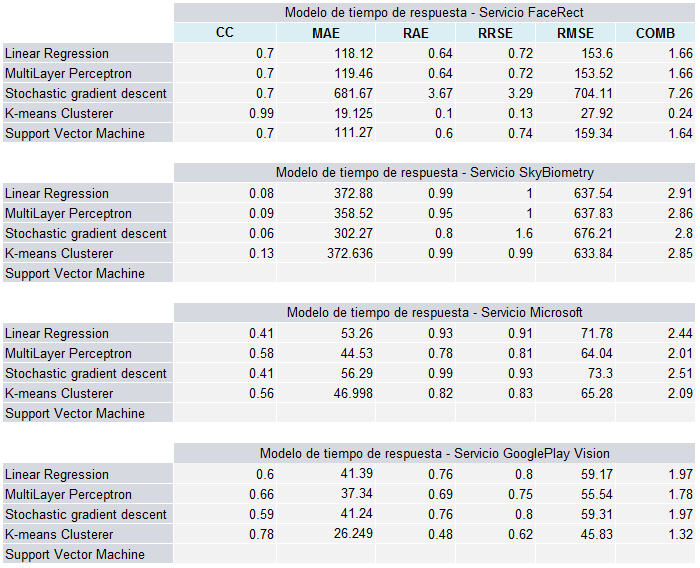
\includegraphics[bb=0bp 0bp 596bp 619bp,scale=0.55]{C:/Users/usuario/Tesisworkspace/Tesis_Standalone/tesis/images/response-face}
\par\end{centering}

\caption{Resultados del atributo ‘Tiempo de respuesta’ para los servicios de
detección de rostros.\label{tab:Resultados-response-face}}
\end{table}


Continuando con la misma línea de análisis, los datos exhibidos demuestran
que el mejor modelo presentado para predecir el tiempo de respuesta
para el problema de detección de rostros es el MultiLayer Perceptron.
El algoritmo no sólo ha arrojado los valores más bajos del error de
predicción sino que en todos los casos, demuestra una buena adaptación
a los dataset que por su naturaleza, difieren en volumen de instancias,
cantidad y tipo de atributos. 

A continuación, se presentan las lineas de predicción para demostrar
el poder de análisis del modelo.

\begin{figure}[H]
\begin{centering}
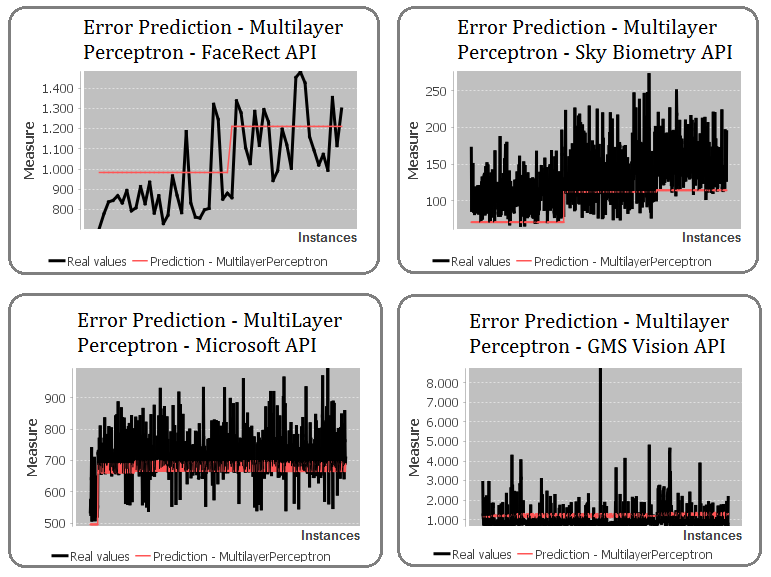
\includegraphics[scale=0.3]{C:/Users/usuario/Tesisworkspace/Tesis_Standalone/tesis/images/response_face_lc}
\par\end{centering}

\caption{Figura comparativa de las predicciones realizadas por el MultiLayer
Perceptron}
\end{figure}



\subsection{Discusión}

En esta sección se contrastaran los escenarios y las técnicas entre
sí mediante las métricas en las cuales se centró el estudio realizado.
Es importante destacar algunas consideraciones sobre el modelo \ac{SMO},
por lo cual se excluyó del análisis. El desempeño de este algoritmo
es predominantemente superior en la calidad de sus respuestas, sin
embargo presenta algunas limitaciones para su uso; el modus operandi
del algoritmo no es apto para formatos de dataset de cientos de instancias
y múltiples atributos, ya que en algunos casos el costo operacional
requirió más de un día de ejecución y en otros casos, sus resultados
no pudieron ser visualizados. 

\begin{table}[H]
\resizebox{.80\textwidth}{!}{%
\begin{tabular*}{20cm}{@{\extracolsep{\fill}}|c|c|c|c|c|c|c|c|c|c|c|c|}
\hline 
\selectlanguage{english}%
\selectlanguage{english}%
 & \multicolumn{4}{c|}{Escenario 1} & \multicolumn{3}{c|}{Escenario 2} & \multicolumn{4}{c|}{Escenario 3}\tabularnewline
\hline 
\selectlanguage{english}%
\selectlanguage{english}%
 & Sin RenderScript K3 & Sin RenderScript S3 & K3 & S3 & S4 & S5 & S6 & FaceRect & SkyBiometry & Microsoft & GMS\tabularnewline
\hline 
Linear Regression & 0.91 & 0.92 & 0.87 & 0.87 & 0.72 & 0.72 & 0.71 & 0.7 & 0.08 & 0.41 & 0.6\tabularnewline
\hline 
MultiLayer Perceptron & 0.99 & 1 & 0.99 & 1 & 1 & 1 & 1 & 0.7 & 0.09 & 0.58 & 0.66\tabularnewline
\hline 
\ac{SGD} & 0.89 & 0.91 & 0.87 & 0.87 & 0.65 & 0.65 & 0.62 & 0.7 & 0.06 & 0.41 & 0.59\tabularnewline
\hline 
Clusterer &  0.98 &  0.98 &  0.99  &  0.99  &  0.63  &  0.58  &  0.65  &  0.99  &  0.13  &  0.56  &  0.78 \tabularnewline
\hline 
\end{tabular*}}

\caption{Especificaciones de los dispositivos móviles utilizados. \label{tab:CC-results}}
\end{table}


A partir de los resultados expuestos, se analiza el impacto de la
calidad de las entradas en el Coeficiente de correlación de los datos.
El primer escenario centralizó la formación de los datasets exclusivamente
en las propiedades inherentes de la entrada del problema. La naturaleza
de los problemas de tipo P, como el escenario 1, conlleva a que el
tiempo de resolución de los mismos dependa exclusivamente de la cantidad
de atributos del problema. Ambas consideraciones suponen un alto grado
de correlación y los datos obtenidos lo confirman.

En contraste, el escenario 3 no consideró propiedades de la entrada
del problema, lo que supone un grado de correlación menor. La entrada
del problema no es fácilmente cuantificable de forma exacta, por lo
que no fueron consideradas como variables para la predicción. Asimismo,
los atributos del dataset son conformados por variables booleanas
que representan los detalles requeridos del servicio, lo que conlleva
a una gran homogeneización de los datos. En consecuencia, dos instancias
análogas en sus requerimientos podrían producir predicciones diferentes
lo cual rompe el criterio de unicidad de toda función matemática.

El caso más cercano al ideal es el escenario 2, en el cual se considera
solo un rasgo de la entrada y un rasgo del componente, conformando
un conjunto acotado de valores y permitiendo que el modelo alcance
una función de correlación estable.

\begin{table}[H]
\resizebox{.80\textwidth}{!}{%
\begin{tabular*}{20cm}{@{\extracolsep{\fill}}|c|c|c|c|c|c|c|c|c|c|c|c|}
\hline 
\selectlanguage{english}%
\selectlanguage{english}%
 & \multicolumn{4}{c|}{Escenario 1} & \multicolumn{3}{c|}{Escenario 2} & \multicolumn{4}{c|}{Escenario 3}\tabularnewline
\hline 
\selectlanguage{english}%
\selectlanguage{english}%
 & Sin RenderScript K3 & Sin RenderScript S3 & K3 & S3 & S4 & S5 & S6 & FaceRect & SkyBiometry & Microsoft & GMS\tabularnewline
\hline 
Linear Regression & 0.02 & 0.03 & 0.03 & 0.03 & 7.72 & 3.69 & 2.06 & 153.6  & 637.54 & 71.78 & 59.17\tabularnewline
\hline 
MultiLayer Perceptron & 0.01 & 0.01 & 0.01 & 0.01 & 1.02 & 0.2 & 0.13 & 153.52 & 637.83  & 64.04 & 55.54\tabularnewline
\hline 
\ac{SGD} & 0.03 & 0.03 & 0.03 & 0.03 & 9.48 & 4.54 & 2.58 & 704.11 & 676.21 & 73.3 & 59.31\tabularnewline
\hline 
Clusterer &  0.01  &  0.01  &  0.01  &  0.01  &  8.67  &  4.36  &  2.2  &  27.92  &  633.84  &  65.28  &  45.83 \tabularnewline
\hline 
\end{tabular*}}

\caption{Especificaciones de los dispositivos móviles utilizados. \label{tab:RMSE-results}}
\end{table}


Considerando el análisis previo y los valores de \ac{RMSE} presentados
en la tabla \ref{tab:RMSE-results}, se sustentan las conclusiones
y suposiciones planteadas anteriormente. Cuanto mayor sea la correlación
entre los datos de entrada del problema y el tiempo de respuesta,
menor es el grado de error en la predicción ya que es más factible
que el modelo encuentre una formula matemática que describa la salida
a partir de la entrada.

Teniendo en cuenta lo visto hasta ahora, el escenario 2 es el que
mejor satisface los requerimientos necesarios para obtener un buen
modelo predictivo ya que las entradas y los componentes son descriptos
en su justa medida. Por lo tanto, a partir de este escenario se desprende
que el modelo LinearRegression es el que mejor se ajusta a los objetivos
del trabajo planteado siempre que el conjunto de datos sea descripto
de forma completa y eficiente. El modelo no presenta efectos de overfit
o underfit sobre los datos garantizando buenos resultados en un futuro
dataset o escenario.

En situaciones desfavorables donde se cuenta con un dataset incompleto
o con sólo datos del componente que se desea analizar, es conveniente
el uso del modelo MultiLayer Perceptron ya que garantiza un analisis
más profundo de los datos. Este análisis intensivo se debe a la idea
intrínseca del algoritmo Neural Network que permite la conjunción
de entradas conformando otras nuevas y facilitando nuevos datos que
no estaban presentes de forma explicita en el dataset. Se estima que
el modelo será capaz de generar buenas estimaciones a un costo temporal
aceptable, lo que significa que la ejecución de un dataset de cientos
de instancias y diversos atributos, no sólo arrojará un resultado
(ventaja frente a otros modelos) sino que la visualización de la respuesta
conllevará a lo sumo una hora de tiempo. 


\section{Conclusiones \label{sec:Conclusiones}}

En este capítulo se presentaron los distintos ambientes de pruebas
y se analizaron los resultados producto de los mismos. En la primera
sección se describió el procedimiento llevado a cabo para la evaluación
de la calidad de los modelos predictivos que aplican algoritmos de
regresión. Luego, se describieron los escenarios que conforman cada
uno de los casos de estudio, donde toma lugar el enfoque propuesto
para la herramienta implementada. 

Finalmente, se exponen los resultados acerca del error de predicción
de los modelos, que indican principalmente tres consideraciones: 
\begin{itemize}
\item En situaciones de conjuntos de datos completos en su estructura, el
modelo Linear Regression es el más conveniente para predecir el tiempo
de respuesta en una aplicación móvil.
\item En contraste, en conjuntos de datos pobres, el modelo MultiLayer Perceptron
adquiere una mejor generalización de los datos, adaptándose a diferentes
formatos de dataset, y diferentes operaciones de componentes.
\item En caso de dataset formados por pocas instancias, el comportamiento
del \ac{SMO} es similar al del Multilayer Perceptron. Sin embargo,
es importante destacar el efecto de overfit de ambos algoritmos, y
particularmente el tiempo de procesamiento que requiere el \ac{SMO}. \end{itemize}

